\subsection{Introducción:}

En este ejercicio vamos a setear las interrupciones basicas, osea las reservadas para el procesador. Para esto completaremos la \textit{IDT}. Se pide que realizemos lo siguiente :

\begin{itemize}
\item [\textit{a)}] Completar la \textit{IDT} de tal forma que indique por pantalla el problema que se produjo y que interrumpa la ejecución.
\item [\textit{b)}] Cargar la  \textit{IDT} y probarla.
\end{itemize}

\subsection{Ítem a): Setear la \textit{IDT}}

Para esto utilizamos los siguientes archivos dados por la catedra   \textit{idt.c}, \textit{isr.h}, \textit{isr.asm} y los completamos. 

 \subsubsection{{\large \textit{Idt.c:}}}
 En este archivo se encuentra la función \textit{IDT\_ENTRY(número, dpl)} la cual recive el numero de la interrupción y su prioridad. La misma se encontraba incompleta y necesitaba ser completada con la información necesaria. La llenamos agregandole el segmento correspondiente y los atributos correpondientes. El segmento que le correpondia se ubicaba en la direccion 0x40 (explicado en el ejercicio 1) y los atributos son los correpondientes a el valor  0x8700, ya que el formato de los atributos de una interrupcion debe ser de la siguiente forma:

 \begin{figure}[H]
\begin{center}
\minipage{0.6\textwidth}
  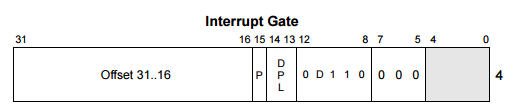
\includegraphics[width=\linewidth]{ejercicio2/interrupcion.png}
  \caption{{\small Formato de los atributos de una interrupcion} }
\endminipage
\end{center}
\end{figure}

Entonces como 0x8E00 representa en binario 1000 1110 0000 0000, tiene el formato que queremos. Ya que P debe ser 1, DPL debe ser 00, luego sigue un 0, luego D (que en este caso es 1 ya que estamos trabajando en 32bits) luego siguen dos unos y por último nueve ceros, lo cual forma el número que queremos. De esta forma nos queda la funcion \textit{IDT\_ENTRY} de la siguiente manera:

 \begin{figure}[H]
\begin{center}
\minipage{1.0\textwidth}
  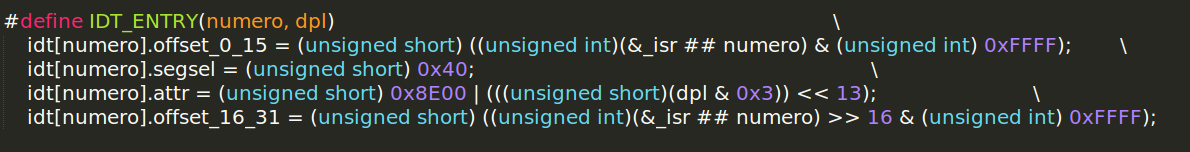
\includegraphics[width=\linewidth]{ejercicio2/idtentry.png}
  \caption{{\small Formato de los atributos de una interrupcion} }
\endminipage
\end{center}
\end{figure}

Por último, creamos las 20 interrupciones correspondientes utilizando \textit{IDT\_ENTRY}  .

 \begin{figure}[H]
\begin{center}
\minipage{0.6\textwidth}
  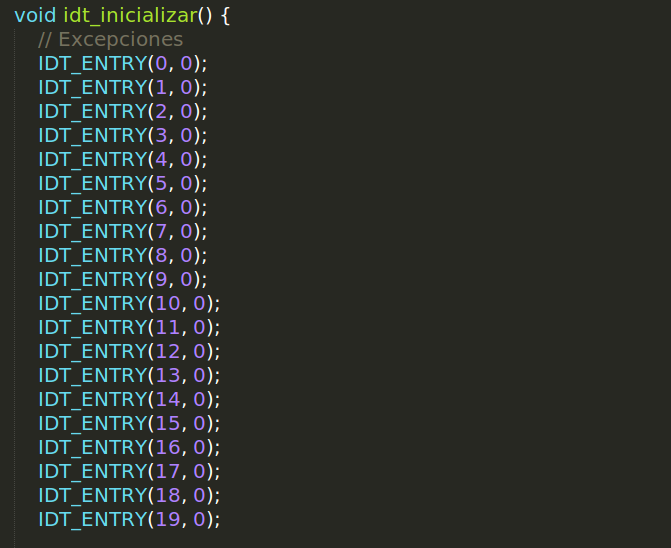
\includegraphics[width=\linewidth]{ejercicio2/idt.png}
  \caption{{\small Formato de los atributos de una interrupcion} }
\endminipage
\end{center}
\end{figure}
 \subsubsection{{\large \textit{Isr.h:}}}

 En este archivo tuvimos que declarar las siguientes funciones:
  \begin{figure}[H]
\begin{center}
\minipage{0.8\textwidth}
  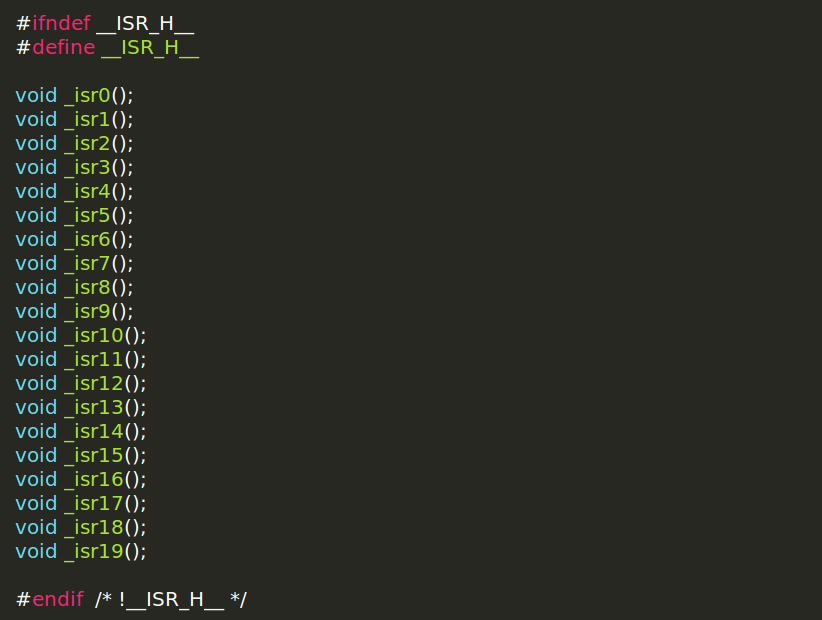
\includegraphics[width=\linewidth]{ejercicio2/isrh.png}
  \caption{{\small Formato de los atributos de una interrupcion} }
\endminipage
\end{center}
\end{figure}


 Sino, la función del archivo anterior, \textit{IDT\_ENTRY}, no compilaba, pues no las encontraba. No es necesario que estas funciones hagan algo, ya que en realidad \textit{IDT\_ENTRY} las utilizaba como macro.

 \subsubsection{{\large \textit{Isr.asm:}}}

Por último, en este archivo, atendemos las interrupciones con sus correspondientes rutinas, como en el enunciado solo se pide que se interrumpa la ejecucion del programa y se muestre por pantalla la iterrupcion que genero el problema, solamente utilizamos una funcion macro dada por la catedra que simplemente muestra dicho mensaje y ejecuta un loop infinito.\\

La macro es la siguiente:
  \begin{figure}[H]
\begin{center}
\minipage{0.6\textwidth}
  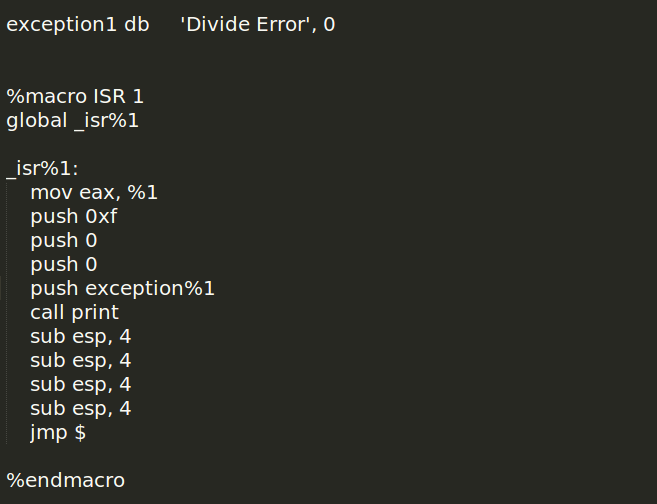
\includegraphics[width=\linewidth]{ejercicio2/macro.png}
  \caption{{\small Macro para atender interrupciones} }
\endminipage
\end{center}
\end{figure}

La macro de la imágen anterior reemplaza  \%1 por el primer parametro que recibe. Este parametro es el número correpsondiente a la interrupción, por ende cuando llegue la interrupucion $"x"$, se pushea el mensaje exception$"x"$ y print muestra por pantalla el mensaje correspondiente a la etiqueta exception$"x"$, para luego quedarse saltando infinitamente y por lo tanto interrupiendo la ejecucion del programa. En la imagen se muestra un ejemplo del mensaje que se mostraria si se produjera la interrupcion 1 , correspondiente a la division por cero.\\

Por ultimo escribimos la rutina de atencion de interrupciones, la cual simplemente llama a la macro anterior, tomando como parámetro el número de la interrupcion.

  \begin{figure}[H]
\begin{center}
\minipage{0.4\textwidth}
  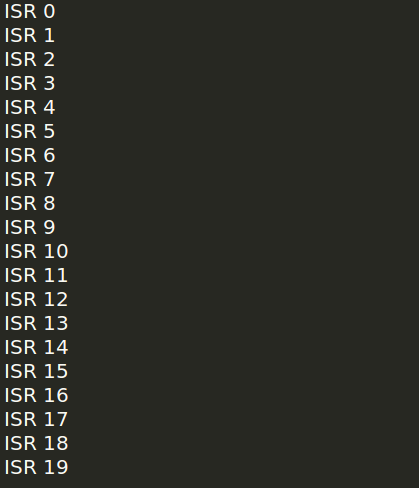
\includegraphics[width=\linewidth]{ejercicio2/israsm.png}
  \caption{{\small Rutina de atencion de interrrupciones.} }
\endminipage
\end{center}
\end{figure}


\subsection{Ítem b): Cargar y probar \textit{IDT}}

Para cargar la \textit{IDT} y probarla, agregamos las siguientes lineas al \textit{kernel}:

\begin{center}
    lidt [IDT\_DESC]\\
    mov eax, 0  $~~~~~~~$  \\
    mov ecx, 1 $~~~~~~~$    \\
    div ecx$~~~~~~~~~~~~~$
\end{center}

Obteniendo el resultado esperado:

  \begin{figure}[H]
\begin{center}
\minipage{0.8\textwidth}
  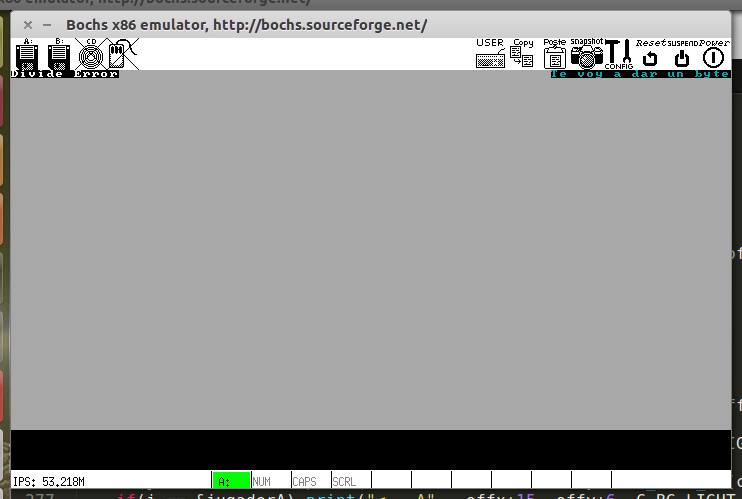
\includegraphics[width=\linewidth]{ejercicio2/division.jpg}
  \caption{{\small Rutina de atencion de interrrupciones.} }
\endminipage
\end{center}
\end{figure}

